\section{Application Context and Requirements}
\label{sec:application}

Firefighter incident command provides a concrete example of the broader class of multi-human digital support settings outlined in the previous section. In this setting, the command-support system is not meant to converse with a single user in isolation. Instead, it supports shared coordination by helping incident command maintain an explicit, inspectable view of operational task state as evidence arrives through multi-party radio traffic. We use this case not as the whole claim of the paper, but as a demanding setting from which to derive requirements for one bounded coordination-support capability.

\subsection{Application Setting}

The user-facing surface is a dashboard that presents the task list together with current task status and recent communication context, as illustrated in Figure~\ref{fig:dashboard}. Its role is to reduce memory burden and preserve an explicit overview of open and completed tasks. The dashboard thus serves as the interface of a bounded information-processing support system for the command team. It helps keep tasks from getting lost in noisy, interleaved, time-critical radio communication.

\begin{figure*}[t]
  \centering
  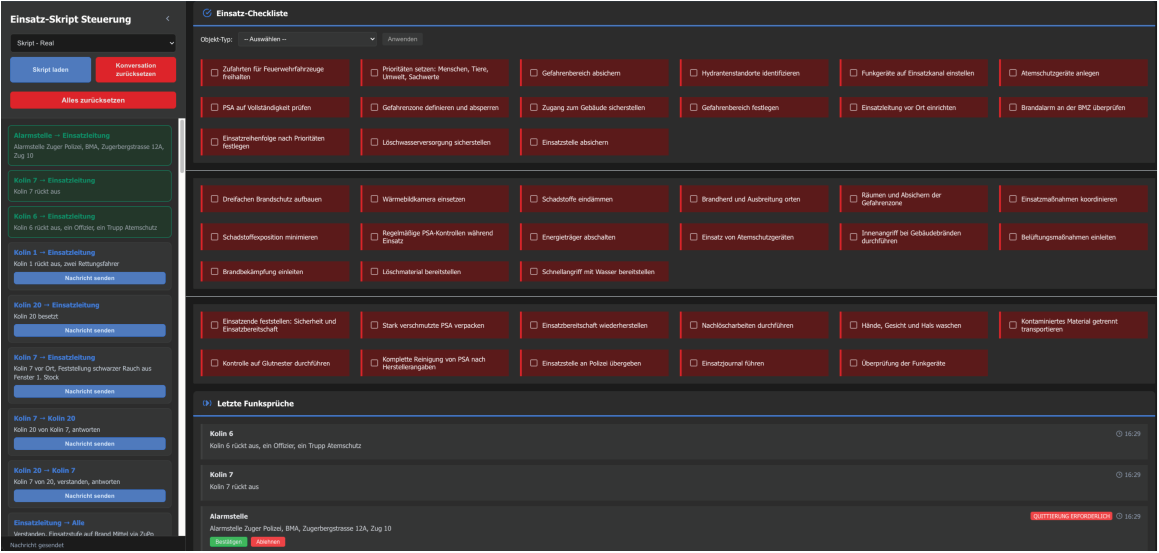
\includegraphics[width=\textwidth]{figures/figure_dashboard.png}
  \caption{Dashboard interface of our command-support system.}
  \label{fig:dashboard}
\end{figure*}

Figure~\ref{fig:workflow} situates this dashboard within our implemented command-support system. In the operational setting, predefined tasks originate from procedures and incident context, for example from baseline checklists associated with the incident type, from object-specific information, and from a building register. This information is available and selected at dispatch time. Radio communication then provides the dynamic evidence for whether those tasks have been assigned to firefighter units, acknowledged, and completed. The present paper therefore treats task-state monitoring as a closed-world problem: the task set is supplied in advance, and transcript evidence is used to update task state.

This application framing is also consistent with lightweight qualitative feedback from a prototype demonstration of our command-support system with active firefighters. Beyond transcript capture itself, they emphasized the value of temporal tracking features, such as seeing how long a task has remained open or how long a crew has been silent. We treat this feedback as informal practitioner grounding rather than as a formal user-study result.

\begin{figure*}[t]
  \centering
  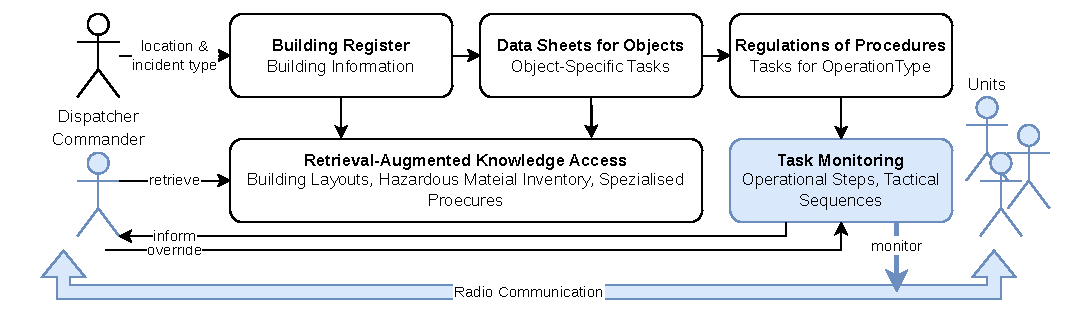
\includegraphics[width=0.92\textwidth]{figures/figure_workflow.pdf}
  \caption{Operational flow of our command-support system, with dashboard components shown in blue.}
  \label{fig:workflow}
\end{figure*}

\subsection{Monitoring Problem}

Emergency radio communication differs substantially from the dialogue structure often assumed in conversational NLP. Messages are short, domain-specific, and often elliptical. Operational meaning is distributed across acknowledgements, updates, and follow-up reports rather than contained in a single self-sufficient utterance. For the command-support system, useful support therefore depends on reconstructing task state from distributed conversational evidence rather than isolated turns.

This creates the concrete design pressure behind our research question. If the dashboard requires speaker identities, the implementation may depend on diarization or prior speaker models despite radio-channel noise and changing crews \citep{Mehrish2023A}. If it requires semantically well-formed utterance boundaries, pause-based segmentation may be insufficient and additional speaker-change or semantic segmentation steps may be needed before task monitoring can run \citep{Mehrish2023A}. These components increase engineering effort and add latency, which is a relevant concern in real-time speech systems that must trade off model complexity against computational load \citep{Michelsanti2020An}. In our setting, such components may fail precisely in the noisy conditions where operational support is most valuable. We therefore investigate how much structure the transcript representation actually needs for this monitoring task. More broadly, the firefighter case can thus be understood as one example of a digital support system that performs a bounded, process-relevant information-processing function inside a human team.

\subsection{System Requirements}

The command-support system must monitor the state of predefined operational tasks supplied from procedures and incident context. The scope is therefore closed-world monitoring of known tasks rather than open-ended task discovery.

The command-support system must operate under explicit human oversight. Proposed task-state updates must remain transparent to the command team and be subject to human confirmation or override.

The command-support system must support near-real-time dashboard updates during ongoing incidents. Task-state information must be revised as new communication evidence becomes available so that the dashboard remains a current operational overview.

\subsection{Task Formulation}

These application requirements lead to a closed-world task formulation. For each predefined task $\tau$ and each discrete prefix index $k$, the model outputs a structured task-state prediction
\[
y(\tau, k) = (a, u, c, o).
\]
Here, $k$ denotes the current transcript prefix, that is, the communication evidence available up to that point. The tuple components correspond to \texttt{assigned}, \texttt{assigned\_unit}, \texttt{completed}, and \texttt{completion\_outcome}, respectively. \texttt{assigned} (boolean) indicates whether the transcript provides evidence that responsibility for the task has been assigned to a unit and acknowledged. \texttt{assigned\_unit} (nullable string) indicates which unit is identified as responsible for the task. \texttt{completed} (boolean) indicates whether the transcript provides evidence that the task has been completed. \texttt{completion\_outcome} (nullable string) captures the reported completion result or completion evidence in short textual form.
